%%%%%%%%%%%%%%%%%%%%%%%%%%%%%%%%%%%%%%%%%%%%%%%%%%%%%%%%%%%%%%%%%%%%%%%%%%%%%%%%%%%%%%%%%%%%%%%%%%%%%%%%%%%%%%%%%%%%%%%%%%%%%%%%%%%%%%%%%%%%%%%%%%%%%%%%%%%%%%%%%%%
% Written By Michael Brodskiy
% Class: Electricity & Magnetism
% Professor: D. Wood
%%%%%%%%%%%%%%%%%%%%%%%%%%%%%%%%%%%%%%%%%%%%%%%%%%%%%%%%%%%%%%%%%%%%%%%%%%%%%%%%%%%%%%%%%%%%%%%%%%%%%%%%%%%%%%%%%%%%%%%%%%%%%%%%%%%%%%%%%%%%%%%%%%%%%%%%%%%%%%%%%%%

\include{Includes.tex}

\title{Homework 10}
\date{December 6, 2023}
\author{Michael Brodskiy\\ \small Professor: D. Wood}

\begin{document}

\maketitle

\begin{enumerate}

  \item As a simplified model of a planet being bombarded with cosmic rays at the poles, consider a conducting sphere of radius $R$ that is being charged with wires at the north and south poles that each have a current $I/2$ flowing onto the sphere, so that the total charge of the sphere is increasing with time $\left( \frac{dQ}{dt}=I \right)$.  Assume the charge is always distributed uniformly on the surface of the sphere.

    \begin{enumerate}

      \item Calculate the displacement current density just above the surface of the sphere.

    We can begin by finding a relationship between displacement current and the electric displacement:

    $$\vec{J}=\frac{\partial \vec{D}}{\partial t}\to\varepsilon_o\frac{\partial\vec{E}}{\partial t}$$

    We know the formula for the electric field to be:

    $$\vec{E}=\frac{Q}{4\pi\varepsilon_o R^2}$$

    Thus, we may conclude:

    $$\vec{J}=\frac{\varepsilon_o}{4\pi\varepsilon_o R^2}\left( \frac{\partial Q}{\partial t} \right)$$
    $$\boxed{\vec{J}=\frac{I}{4\pi R^2}}$$

      \item Use the Amp\`re-Maxwell equation to calculate the induced magnetic field just above the surface at location that is an angle $\theta$ from the north pole (latitude = $90^{\circ}-\theta$). [Hint: Use a ring of constant latitude as the amperian loop and use a cap-shaped enclosed surface of the loop that follows the surface of the sphere. Be sure to include both the physical current and the displacement current.]  (While this is an interesting calculation, note that this is not a significant contribution to the Earth’s magnetic field.)

        We may begin by expressing the equation as:

        $$\int \vec{B}\cdot d\vec{l}=\mu_o\left( \sum I \right)$$
        $$\vec{B}\int d\vec{l}=\mu_o\left( I+I_d \right)$$

        The situation can be sketched as follows:

        \begin{figure}[h]
          \centering
          \tikzset{every picture/.style={line width=0.75pt}} %set default line width to 0.75pt        

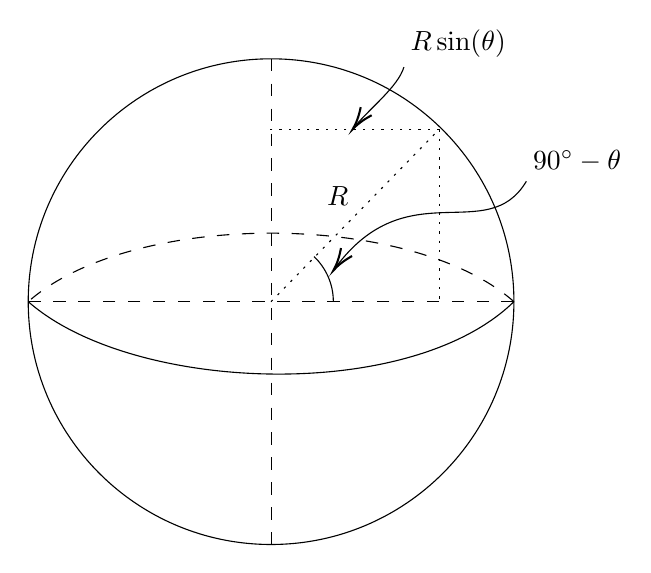
\begin{tikzpicture}[x=0.75pt,y=0.75pt,yscale=-1,xscale=1]
%uncomment if require: \path (0,485); %set diagram left start at 0, and has height of 485

%Shape: Circle [id:dp4936381296702055] 
\draw   (179,157) .. controls (179,92.38) and (231.38,40) .. (296,40) .. controls (360.62,40) and (413,92.38) .. (413,157) .. controls (413,221.62) and (360.62,274) .. (296,274) .. controls (231.38,274) and (179,221.62) .. (179,157) -- cycle ;
%Curve Lines [id:da7684497988482555] 
\draw    (179,157) .. controls (229,201) and (363,206) .. (413,157) ;
%Curve Lines [id:da031906274558686665] 
\draw  [dash pattern={on 4.5pt off 4.5pt}]  (413,157) .. controls (363,113) and (229,113) .. (179,157) ;
%Straight Lines [id:da7237618188990222] 
\draw  [dash pattern={on 4.5pt off 4.5pt}]  (296,40) -- (296,274) ;
%Straight Lines [id:da6805862140011472] 
\draw  [dash pattern={on 4.5pt off 4.5pt}]  (413,157) -- (179,157) ;
%Straight Lines [id:da6636715436204372] 
\draw  [dash pattern={on 0.84pt off 2.51pt}]  (296,157) -- (377,74) ;
%Shape: Arc [id:dp03958996945390081] 
\draw  [draw opacity=0] (316.72,135.3) .. controls (322.44,140.76) and (326,148.47) .. (326,157) -- (296,157) -- cycle ; \draw   (316.72,135.3) .. controls (322.44,140.76) and (326,148.47) .. (326,157) ;  
%Curve Lines [id:da7315028520131872] 
\draw    (419,99) .. controls (400.19,130.68) and (361.78,93.75) .. (327.05,140.56) ;
\draw [shift={(326,142)}, rotate = 305.54] [color={rgb, 255:red, 0; green, 0; blue, 0 }  ][line width=0.75]    (10.93,-3.29) .. controls (6.95,-1.4) and (3.31,-0.3) .. (0,0) .. controls (3.31,0.3) and (6.95,1.4) .. (10.93,3.29)   ;
%Straight Lines [id:da960505724523711] 
\draw  [dash pattern={on 0.84pt off 2.51pt}]  (377,74) -- (377,157.42) ;
%Straight Lines [id:da7630353719230638] 
\draw  [dash pattern={on 0.84pt off 2.51pt}]  (377,74) -- (293.58,74) ;
%Curve Lines [id:da15200728730904722] 
\draw    (360,44) .. controls (357.17,53.45) and (343.61,63.79) .. (336.47,72.5) ;
\draw [shift={(335.29,74)}, rotate = 306.71] [color={rgb, 255:red, 0; green, 0; blue, 0 }  ][line width=0.75]    (10.93,-3.29) .. controls (6.95,-1.4) and (3.31,-0.3) .. (0,0) .. controls (3.31,0.3) and (6.95,1.4) .. (10.93,3.29)   ;

% Text Node
\draw (421,95.6) node [anchor=south west] [inner sep=0.75pt]    {$90^{\circ } -\theta $};
% Text Node
\draw (334.5,112.1) node [anchor=south east] [inner sep=0.75pt]    {$R$};
% Text Node
\draw (362,40.6) node [anchor=south west] [inner sep=0.75pt]    {$R\sin( \theta )$};


\end{tikzpicture}

          \caption{The $90^{\circ}-\theta$ Shift Switches $\cos\to\sin$}
          \label{fig:1}
        \end{figure}

        We can then express the path as:

        $$\vec{B}(2\pi R\sin(\theta))=\mu_o(I+JA)$$
        $$\vec{B}(2\pi R\sin(\theta))=\mu_o(I+I)$$

        And finally, we get:

        $$\boxed{\vec{B}=\frac{\mu_o I}{\pi R\sin(\theta)}}$$

    \end{enumerate}

  \item Consider a capacitor with circular parallel plates of radius $a$ and separation $d$, where $d<<a$, there the capacitor is discharging with a current $I$.

    \begin{enumerate}

      \item Find the Poynting vector in the space between the plates. Assume that the surface charge is distributed uniformly over the plates.

        We may find the Poynting vector using the relation:

        $$\oint \vec{B}\cdot d\vec{A}=\mu_o\varepsilon_o\frac{d}{dt}\oint \vec{E}\cdot d\vec{A}$$

        Given the uniform charge contained within the area as $q$, we may find:

        $$\vec{E}=\frac{\sigma}{\varepsilon_o}$$
        $$\vec{E}=\frac{q}{\pi\varepsilon_o a^2}$$

        From here, we get:

        $$\vec{B}\oint d\vec{r}=\mu_o\varepsilon_o\frac{d}{dt}\left(\frac{q}{\pi\varepsilon_o a^2} \int d\vec{A}\right)$$
        $$\vec{B}(2\pi r)=\mu_o\varepsilon_o\frac{\pi r^2}{\pi\varepsilon_o a^2}\frac{dq}{dt}$$
        $$\vec{B}=\frac{\mu_or}{2\pi a^2}\frac{dq}{dt}$$

        The change in charge with respect to time may be described as the current, so we get:

        $$\vec{B}=\frac{\mu_orI}{2\pi a^2}$$

        We can then find the Poynting vector, using:

        $$\vec{S}=\frac{1}{\mu_o}\left( \vec{E}\cdot\vec{B} \right)\bold{\hat{r}}$$
        $$\vec{S}=\frac{1}{\mu_o}\left( \frac{q}{\pi\varepsilon_o a^2}\cdot\frac{\mu_orI}{2\pi a^2} \right)\bold{\hat{r}}$$

        This finally gives:

        $$\boxed{\vec{S}=\frac{qrI}{2\pi^2\varepsilon_o a^4}\bold{\hat{r}}}$$

      \item Calculate the rates of energy flow out of the volume between the plates by integrating $\vec{S}$ over an appropriate surface and show that it is equal to $|IV|$.

        The energy flow out of the volume may be defined as:

        $$P=\int \vec{S}\,dA$$
        $$P=\vec{S}(2\pi a d)$$

        Plugging in the value from (a) for $\vec{S}$, and evaluating at $r=a$ we get:

        $$P=\left( \frac{qaI}{2\pi^2\varepsilon_o a^4} \right)\left( 2\pi ad \right)$$
        $$P_{in}=\left( \frac{qId}{\pi\varepsilon_o a^2} \right)$$

        The flow out would be the negative equivalent:

        $$\boxed{P_{out}=-\frac{qId}{\pi\varepsilon_o a^2}}$$

        We can see that the voltage may be defined as:

        $$V=\frac{qd}{\pi\varepsilon_o a^2}$$

        And that we then get the power outflow as:

        $$P=-IV=|-IV|$$

    \end{enumerate}

  \item An ideal parallel plate capacitor with area $A$ and separation $d$ is oriented with the lower plate in the $xy$ plane and is immersed in a uniform horizontal magnetic field $\vec{B}=B_o\bold{\hat{x}}$. The capacitor starts with a charge $+Q$ on the lower plate and $−Q$ on the upper plate. At time $t=0$, a vertical wire with resistance $R$ is connected between the plates.

    \begin{enumerate}

      \item Find the momentum (magnitude and direction) stored in the $\vec{E}$ and $\vec{B}$ fields at time $t=0$.

        The magnetic field is given as:

        $$\vec{B}=B_o\bold{\hat{x}}$$

        The electric field can be defined as:

        $$\vec{E}=\frac{Q}{\varepsilon_o A}\bold{\hat{z}}$$

        The momentum density is defined as:

        $$\frac{\vec{P}}{V}=\varepsilon_o\vec{E}\times\vec{B}$$

        With $V=Ad$, we get:

        $$\vec{P}=\varepsilon_oAd\left(\vec{E}\times\vec{B}\right)$$
        $$\vec{P}=\varepsilon_oAd\left(\frac{Q}{\varepsilon_o A}\bold{\hat{z}}\times B_o\bold{\hat{x}}\right)$$
        $$\vec{P}=\varepsilon_oAd\left|\begin{matrix} \bold{\hat{x}} & \bold{\hat{y}} & \bold{\hat{z}}\\ 0 & 0 & \frac{Q}{\varepsilon_o A}\\ B_o & 0 & 0\\ \end{matrix}\right|$$

        Evaluating the matrix, we get:

        $$\vec{P}=\varepsilon_oAd\left( \frac{B_oQ}{\varepsilon_o A} \right)\bold{\hat{y}}$$
        $$\boxed{\vec{P}=dB_oQ\bold{\hat{y}}}$$

      \item Find the force on the wire as a function of time

      \item Find the total impulse $\left( \int\vec{F}\,dt \right)$ on the wire for $t\to\infty$. Compare this with the change in stored momentum.

    \end{enumerate}

  \item We re-revisit the spinning hollow sphere from earlier assignments — a hollow insulating sphere of radius $R$ and mass $M$ centered at the origin is covered with a uniform surface charge $\sigma=Q/(4\pi R^2)$, rotating about the $z$-axis with angular frequency $\omega$. This time we consider both the magnetic field and the electric field produced by the sphere itself.

    \begin{enumerate}

      \item Calculate the total energy of the electric and magnetic fields. You can use the results from Homework 8, Problem 1 for the $\vec{B}$-field — you do not need to re-derive it.  Be sure to include the magnetic field inside the sphere as well as outside.

      \item Calculate the total angular momentum of the electromagnetic fields, $L_Q$.

      \item Consider a spinning shell whose rest energy $(Mc^2)$ is equal to its electrostatic potential energy $(Q^2/(8\pi\varepsilon_o R))$. Find the ratio between the mechanical ($L_M$) and electromagnetic ($L_Q$) contributions to the angular momentum. Use the fact that $c=1/\sqrt{\varepsilon_o\mu_o}$.

    \end{enumerate}

\end{enumerate}

\end{document}

